
\chapter{Evaluation}
\label{cha:evaluation}
In diesen Abschnitt nehmen wir eine Bewertung der einzelnen
Bestandteile der Software vor. Dabei geht es zum einen um die
Client-Server Kommunikation, die Bahnplanung und Kollisionsvermeidung,
und zum Anderen um die Lokalisierung des Clients im Raum mit dem
Partikelfilter und die Ballerkennung.
\section{Evaluierung des Servers}
\label{sec:eval-des-serv}
%\section{Evaluierung des Clients}
\subsection{Lokalisierung mit den Sonar-Partikelfilter}
\label{sec:lokal-mit-den}
Bei unseren Versuchen die Position des Roboters im Raum zu bestimmen,
stiessen wir recht früh auf Probleme: So wurde regelmäßig eine
komplett falsche Position im Raum bestimmt oder aber (gerade wenn der
Roboter sich nahe einer Wand befand) die dem Roboter gegenüberliegende
Position am anderen Ende des Raums als Position erkannt.  Nach
mehreren Versuchen stellten wir schließlich fest, dass die
Lokalisierung besonders zuverlässig war, wenn der Roboter beim Start
des Clients sich in der Mitte des Raums befand, sodass bei der
Initialisierung des Partikelfilters durch die initiale Rotation der
Abstand zu den Wänden zu beiden Seiten gleich war. Um nun der Ursache
dieses Phänomens auf die Spur zu kommen, haben wir dann unser eigenes
Visualisierungsskript geschrieben. Wir beschreiben nun zunächst die
Funktionsweise und Installation des Skriptes, bevor wir uns den
Ergebnissen zuwenden.
\input{visualisierung}

%\input{visualisierung}

%%% Local Variables:
%%% mode: latex
%%% TeX-master: "template"
%%% End:


\section{False Positives bei der Ballerkennung}
\label{sec:false-positives-bei}
Wie bereits im Abschnitt \ref{sec:balldetection} erwähnt, kann es bei
der Ballerkennung zu False Positives kommen. Diese liegen in der
Funktionsweise der Ballerkennung begründet: Nach Aufnahme des
Kamerabildes wird das Bild vom RGB- in den HSV-Farbraum umgewandelt,
der anschließend nach roten Partikeln gefiltert wird. Erreichen diese
einen gewissen Schwellwert, werden diese nach kreisförmigen Objekten
durchsucht. Anschließend wird die Wahrscheinlichkeit berechnet, ob es
sich dabei um einen Ball handelt. Wenn nun aber im Kamerabild so ein
rotes Objekt ist (z.B: Ein anderer p3dx-Roboter), wird dieses mit
hoher Wahrscheinlichkeit als ,,Ball'' erkannt. In unseren Versuchen
wurden unter anderen der Feuerlöscher des Labors, aber auch die roten
Schränke gerne als ,,Bälle'' erkannt. Dies konnten wir durch Aufbau
eines geeigneten Sichtschutzes verhindern, allerdings kam es immer
noch zu false Positives an Stellen, wo weder ein rotes Objekt, noch
sonst irgendein Objekt vorhanden war. Wir konnten schließlich durch
Rückfrage mit Tobias Breuer klären, dass dann höchstwahrscheinlich im
Licht der den Vorraum des Fahrstuhl vor dem Robotiklabor beleuchtenden
Lampen soviele Rot-Partikel vorhanden sind, dass auch da unter
Umständen false Positives auftauchen können. Aus Zeitgründen war es
uns leider nicht mehr möglich zu testen, ob das Ausschalten der Lampen
zu einer Verbesserung geführt hätte. An und für sich wäre das aber die
logische Konsequenz aus der vermuteten Ursache und auch die leichteste
Möglichkeit, diese Vermutung auf ihren Wahrheitsgehalt zu überprüfen.

%%% Local Variables:
%%% mode: latex
%%% TeX-master: "template"
%%% End:


%%% Local Variables:
%%% mode: latex
%%% TeX-master: "template"
%%% End:


%Bei der Kommunikation war zu testen, pob
%\input{eva_kommunikation}
\subsection{Client-Server Kommunikation}
Die zu testende Funktionalität ist das Übermitteln der Zielpunkte der
geplanten Bahn an den Client und der Empfang der Roboterpositionen vom
Client durch den Server. Bei unseren Experimenten traten keinerlei
Probleme auf. 
\subsection{Bahnplanung}
Die Bahnplanung soll ja eine möglichst zufällige Auswahl von Punkten
treffen, sodass die Roboter möglichst viele im Raum verteile
Positionen anfahren, sodass irgendwann der Roboter den Ball nahe genug
kommt, um ihm zu erkennen. Dies leistet die Bahnplanung ohne Probleme.
\subsection{Kollisonsvermeidung}
%Hier waren mehrere Aspekte zu untersuchen
Hier ergab sich das Problem, dass wir bei unseren Versuchen nur
bedingtes Kollisionspotential hatten, da der entsprechende Raum (kaum
Problempotential hatte. Also wurde eine Version des Servers mit einer
alternativen Karte gebaut. Diese Karte repräsentiert einen fiktiven
Raum mit mehreren Zwischenwänden als mögliche Hindernisse. Natürlich
liess sich diese Version aber nicht mit den realen Robotern testen, da
der entsprechende Raum ja eigentlich nicht existiert. Also wurde auf
den im Abschnitt \ref{serv:testclient} auf Seite
\pageref{serv:testclient} beschriebenen Testclient
zurückgegriffen. Damit wurde eine Suche mit drei Robotern simuliert,
die ohne Kollisionen verlief. Abbildung \ref{fig:kollisonsvermeidung}
zeigt die Simulation mit je einer Momentaufnahme für beide Kartenansichten.
%\begin{addmargin}{-1.5cm}
%\begin{nofloat}{figure}%\centering
\begin{figure}[h!]
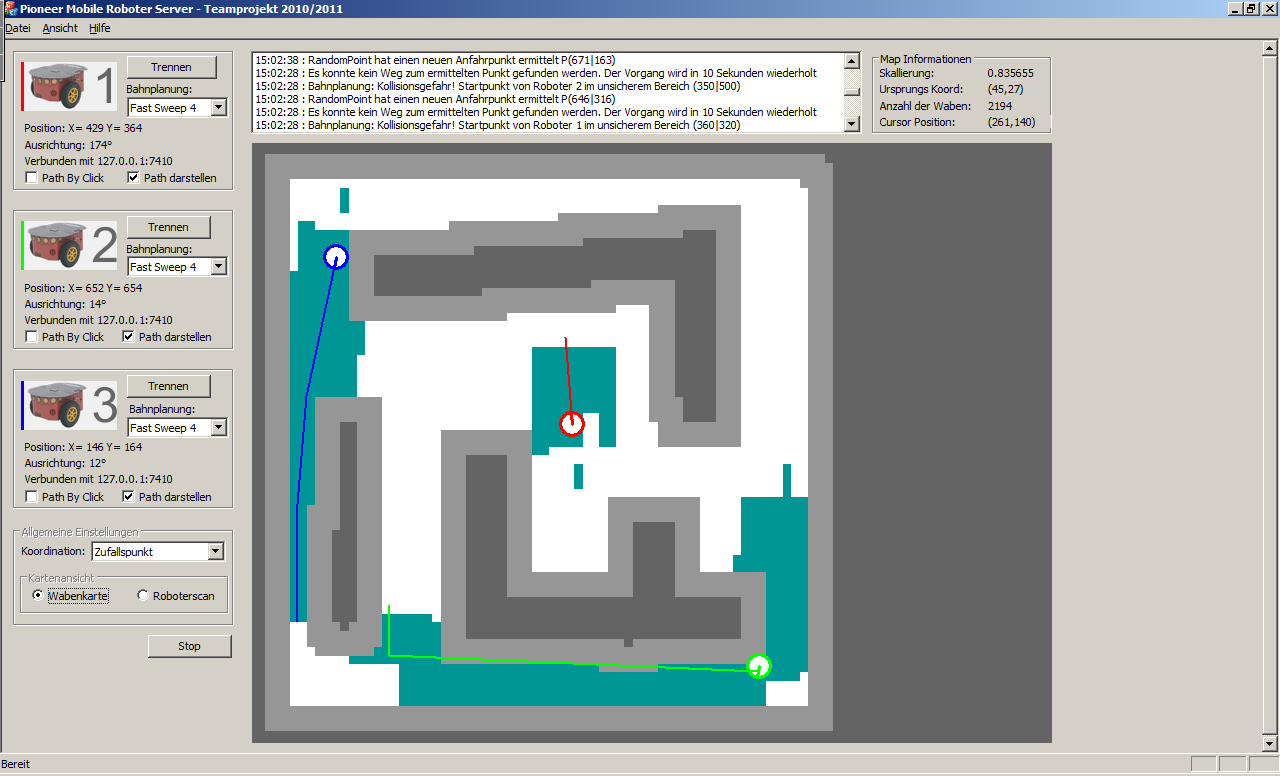
\includegraphics[width=0.5\linewidth]{bilder/avoidCollision2}
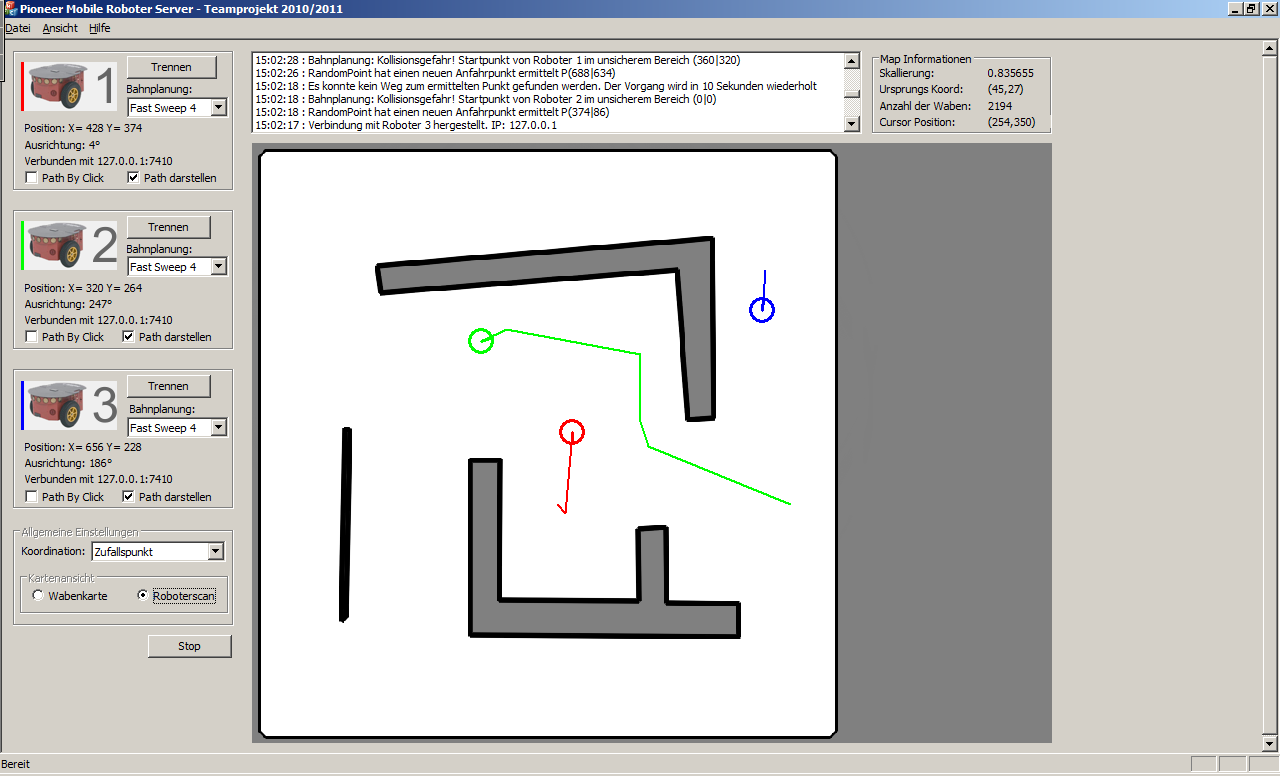
\includegraphics[width=0.5\linewidth]{bilder/avoidCollision1}
\caption{Waben- und Roboterscankarte beim Test der
  Kollisionserkennung}
\label{fig:kollisonsvermeidung}
\end{figure}
%\end{nofloat}
%\end{addmargin}
% Entsprechend arbeiten konnten, da unsere Laptops schon durch den
%ersten Roboter, sowie den Server ,,belegt'' waren. Somit konnten wir
%mit dem realen Roboter nur testen, ob die Kollision mit Wänden
%vermieden wurde. Dies klappte in der Tat ohne Probleme. 
Danach haben wir getestet, ob die Erkennung der Wände auch mit einen
Roboter im Raum vor dem Robotiklabor im Braunschweiger
Informatikzentrum funktionieren würde. Wie oben erwähnt, hatte dieser
deutlich geringeres Problempotential. Wie erwartet klappte dann auch
die Vermeidung der Wände ohne Probleme. Nur einmal wurde eine Wand
doch angefahren. \newpage Dies war darauf zurückzuführen, dass die
Positionserkennung  mit dem Sonar-Partikelfilter kurzfristig einen
Ausreißer hatte (vgl. hierzu auch den Abschnitt
\ref{sec:lokal-mit-den} ab Seite \pageref{sec:lokal-mit-den}). Somit
war aus Sicht der Kollisonsvermeidung keine Gefahr vorhanden und
brauchte somit auch nicht abgewehrt werden. Im Endeffekt ist dieser
,,Fehlschlag'' also kein Zeichen, dass die Kollisionsvermeidung nicht
funktionieren würde. \\\\
%Um nun das Verhalten der Bahnplanung und Kollisionsvermeidung bei
%mehreren Robotern zu testen, wurde auf den im Abschnitt
%\ref{serv:testclient} auf Seite \pageref{serv:testclient}
%beschriebenen Testclient zurückgegriffen, der das Verhalten des
%Clients emuliert. Wir haben insgesamt drei virtuelle Testclients mit
%dem Server verbunden und konnten somit die Kollisionsvermeidung testen.
%Bei der Bahnplanung ergab sich das Problem, dass uns nur ein Roboter
%zum Testen zur Verfügung 
%input{eva_bahnplanung}
%\input{eva_kollision}
%Client-Server Kommunikation, die Bahnplanung und Kollisionsvermei
%%% Local Variables:
%%% mode: latex
%%% TeX-master: "template"
%%% End:

\section{Evaluierung des Clients}
\subsection{Lokalisierung mit den Sonar-Partikelfilter}
\label{sec:lokal-mit-den}
Bei unseren Versuchen die Position des Roboters im Raum zu bestimmen,
stiessen wir recht früh auf Probleme: So wurde regelmäßig eine
komplett falsche Position im Raum bestimmt oder aber (gerade wenn der
Roboter sich nahe einer Wand befand) die dem Roboter gegenüberliegende
Position am anderen Ende des Raums als Position erkannt.  Nach
mehreren Versuchen stellten wir schließlich fest, dass die
Lokalisierung besonders zuverlässig war, wenn der Roboter beim Start
des Clients sich in der Mitte des Raums befand, sodass bei der
Initialisierung des Partikelfilters durch die initiale Rotation der
Abstand zu den Wänden zu beiden Seiten gleich war. Um nun der Ursache
dieses Phänomens auf die Spur zu kommen, haben wir dann unser eigenes
Visualisierungsskript geschrieben. Wir beschreiben nun zunächst die
Funktionsweise und Installation des Skriptes, bevor wir uns den
Ergebnissen zuwenden.
\section{Visualisierung der Partikelmengen des Partikelfilters}
Da die im Partikelfilter integrierte Visualisierung der Partikelmenge
nicht immer funktionierte und es auch keine direkte SPeichermöglichkeit der
 Bilder gab, haben wir den Partikelfilter, so erweitert, dass die
Partikelmenge in eine Datei geschrieben werden kann (
\ref{sec:sonarparticlefilter}) und passend dazu ein Skript (in Python unter
 Benutzung von pygame geschrieben), welches die Partikel anhand der Daten
 aus einer Partikelmengendatei über ein Bild legt. Dieses ist im Ordner
 Visualisierung im SVN-Repository unter dem Namen visualize.py zu finden.

 \subsection{HOWTO: Installieren der Abhängigkeiten des
Visualisierungsskriptes und Benutzung dessen}
 \begin{itemize}
	 \item Python 3.2 herunterladen und installieren\footnote{http://python.org/ftp/python/3.2.2/python-3.2.2.msi}
	 \item pygame 1.9.2a0 für Python 3.2 installieren \footnote{http://pygame.org/ftp/pygame-1.9.2a0.win32-py3.2.msi}
	 \item Python 3.2 zum PATH hinzufügen
	 \item cmd/Eingabeaufforderung öffnen
	 \item In den Ordner Visualisierung des Repositories wechseln
	 \item Das Visualisierungsskript kann nun folgendermaßen benutzt werden:\\
	 		\lstinline|python visualize.py (Dateiname des Bildes) (Dateiname der Partikelmengendatei)| \\
 			z.b. \lstinline|python visualize.py OccuMap.bmp visual.log|
	 \item Das Ausgabebild hat dann den Namen V\_(Dateiname der Partikelmengendatei)\_(Dateiname des Bildes)
\end{itemize}

%\section{Visualisierung der Partikelmengen des Partikelfilters}
Da die im Partikelfilter integrierte Visualisierung der Partikelmenge
nicht immer funktionierte und es auch keine direkte SPeichermöglichkeit der
 Bilder gab, haben wir den Partikelfilter, so erweitert, dass die
Partikelmenge in eine Datei geschrieben werden kann (
\ref{sec:sonarparticlefilter}) und passend dazu ein Skript (in Python unter
 Benutzung von pygame geschrieben), welches die Partikel anhand der Daten
 aus einer Partikelmengendatei über ein Bild legt. Dieses ist im Ordner
 Visualisierung im SVN-Repository unter dem Namen visualize.py zu finden.

 \subsection{HOWTO: Installieren der Abhängigkeiten des
Visualisierungsskriptes und Benutzung dessen}
 \begin{itemize}
	 \item Python 3.2 herunterladen und installieren\footnote{http://python.org/ftp/python/3.2.2/python-3.2.2.msi}
	 \item pygame 1.9.2a0 für Python 3.2 installieren \footnote{http://pygame.org/ftp/pygame-1.9.2a0.win32-py3.2.msi}
	 \item Python 3.2 zum PATH hinzufügen
	 \item cmd/Eingabeaufforderung öffnen
	 \item In den Ordner Visualisierung des Repositories wechseln
	 \item Das Visualisierungsskript kann nun folgendermaßen benutzt werden:\\
	 		\lstinline|python visualize.py (Dateiname des Bildes) (Dateiname der Partikelmengendatei)| \\
 			z.b. \lstinline|python visualize.py OccuMap.bmp visual.log|
	 \item Das Ausgabebild hat dann den Namen V\_(Dateiname der Partikelmengendatei)\_(Dateiname des Bildes)
\end{itemize}

%%% Local Variables:
%%% mode: latex
%%% TeX-master: "template"
%%% End:


\section{False Positives bei der Ballerkennung}
\label{sec:false-positives-bei}
Wie bereits im Abschnitt \ref{sec:balldetection} erwähnt, kann es bei
der Ballerkennung zu False Positives kommen. Diese liegen in der
Funktionsweise der Ballerkennung begründet: Nach Aufnahme des
Kamerabildes wird das Bild vom RGB- in den HSV-Farbraum umgewandelt,
der anschließend nach roten Partikeln gefiltert wird. Erreichen diese
einen gewissen Schwellwert, werden diese nach kreisförmigen Objekten
durchsucht. Anschließend wird die Wahrscheinlichkeit berechnet, ob es
sich dabei um einen Ball handelt. Wenn nun aber im Kamerabild so ein
rotes Objekt ist (z.B: Ein anderer p3dx-Roboter), wird dieses mit
hoher Wahrscheinlichkeit als ,,Ball'' erkannt. In unseren Versuchen
wurden unter anderen der Feuerlöscher des Labors, aber auch die roten
Schränke gerne als ,,Bälle'' erkannt. Dies konnten wir durch Aufbau
eines geeigneten Sichtschutzes verhindern, allerdings kam es immer
noch zu false Positives an Stellen, wo weder ein rotes Objekt, noch
sonst irgendein Objekt vorhanden war. Wir konnten schließlich durch
Rückfrage mit Tobias Breuer klären, dass dann höchstwahrscheinlich im
Licht der den Vorraum des Fahrstuhl vor dem Robotiklabor beleuchtenden
Lampen soviele Rot-Partikel vorhanden sind, dass auch da unter
Umständen false Positives auftauchen können. Aus Zeitgründen war es
uns leider nicht mehr möglich zu testen, ob das Ausschalten der Lampen
zu einer Verbesserung geführt hätte. An und für sich wäre das aber die
logische Konsequenz aus der vermuteten Ursache und auch die leichteste
Möglichkeit, diese Vermutung auf ihren Wahrheitsgehalt zu überprüfen.

%%% Local Variables:
%%% mode: latex
%%% TeX-master: "template"
%%% End:


%%% Local Variables:
%%% mode: latex
%%% TeX-master: "template"
%%% End:

%\subsection{Lokalisierung mit den Sonar-Partikelfilter}
\label{sec:lokal-mit-den}
Bei unseren Versuchen die Position des Roboters im Raum zu bestimmen,
stiessen wir recht früh auf Probleme: So wurde regelmäßig eine
komplett falsche Position im Raum bestimmt oder aber (gerade wenn der
Roboter sich nahe einer Wand befand) die dem Roboter gegenüberliegende
Position am anderen Ende des Raums als Position erkannt.  Nach
mehreren Versuchen stellten wir schließlich fest, dass die
Lokalisierung besonders zuverlässig war, wenn der Roboter beim Start
des Clients sich in der Mitte des Raums befand, sodass bei der
Initialisierung des Partikelfilters durch die initiale Rotation der
Abstand zu den Wänden zu beiden Seiten gleich war. Um nun der Ursache
dieses Phänomens auf die Spur zu kommen, haben wir dann unser eigenes
Visualisierungsskript geschrieben. Wir beschreiben nun zunächst die
Funktionsweise und Installation des Skriptes, bevor wir uns den
Ergebnissen zuwenden.
\section{Visualisierung der Partikelmengen des Partikelfilters}
Da die im Partikelfilter integrierte Visualisierung der Partikelmenge
nicht immer funktionierte und es auch keine direkte SPeichermöglichkeit der
 Bilder gab, haben wir den Partikelfilter, so erweitert, dass die
Partikelmenge in eine Datei geschrieben werden kann (
\ref{sec:sonarparticlefilter}) und passend dazu ein Skript (in Python unter
 Benutzung von pygame geschrieben), welches die Partikel anhand der Daten
 aus einer Partikelmengendatei über ein Bild legt. Dieses ist im Ordner
 Visualisierung im SVN-Repository unter dem Namen visualize.py zu finden.

 \subsection{HOWTO: Installieren der Abhängigkeiten des
Visualisierungsskriptes und Benutzung dessen}
 \begin{itemize}
	 \item Python 3.2 herunterladen und installieren\footnote{http://python.org/ftp/python/3.2.2/python-3.2.2.msi}
	 \item pygame 1.9.2a0 für Python 3.2 installieren \footnote{http://pygame.org/ftp/pygame-1.9.2a0.win32-py3.2.msi}
	 \item Python 3.2 zum PATH hinzufügen
	 \item cmd/Eingabeaufforderung öffnen
	 \item In den Ordner Visualisierung des Repositories wechseln
	 \item Das Visualisierungsskript kann nun folgendermaßen benutzt werden:\\
	 		\lstinline|python visualize.py (Dateiname des Bildes) (Dateiname der Partikelmengendatei)| \\
 			z.b. \lstinline|python visualize.py OccuMap.bmp visual.log|
	 \item Das Ausgabebild hat dann den Namen V\_(Dateiname der Partikelmengendatei)\_(Dateiname des Bildes)
\end{itemize}

%\section{Visualisierung der Partikelmengen des Partikelfilters}
Da die im Partikelfilter integrierte Visualisierung der Partikelmenge
nicht immer funktionierte und es auch keine direkte SPeichermöglichkeit der
 Bilder gab, haben wir den Partikelfilter, so erweitert, dass die
Partikelmenge in eine Datei geschrieben werden kann (
\ref{sec:sonarparticlefilter}) und passend dazu ein Skript (in Python unter
 Benutzung von pygame geschrieben), welches die Partikel anhand der Daten
 aus einer Partikelmengendatei über ein Bild legt. Dieses ist im Ordner
 Visualisierung im SVN-Repository unter dem Namen visualize.py zu finden.

 \subsection{HOWTO: Installieren der Abhängigkeiten des
Visualisierungsskriptes und Benutzung dessen}
 \begin{itemize}
	 \item Python 3.2 herunterladen und installieren\footnote{http://python.org/ftp/python/3.2.2/python-3.2.2.msi}
	 \item pygame 1.9.2a0 für Python 3.2 installieren \footnote{http://pygame.org/ftp/pygame-1.9.2a0.win32-py3.2.msi}
	 \item Python 3.2 zum PATH hinzufügen
	 \item cmd/Eingabeaufforderung öffnen
	 \item In den Ordner Visualisierung des Repositories wechseln
	 \item Das Visualisierungsskript kann nun folgendermaßen benutzt werden:\\
	 		\lstinline|python visualize.py (Dateiname des Bildes) (Dateiname der Partikelmengendatei)| \\
 			z.b. \lstinline|python visualize.py OccuMap.bmp visual.log|
	 \item Das Ausgabebild hat dann den Namen V\_(Dateiname der Partikelmengendatei)\_(Dateiname des Bildes)
\end{itemize}

%%% Local Variables:
%%% mode: latex
%%% TeX-master: "template"
%%% End:

%\section{Visualisierung der Partikelmengen des Partikelfilters}
Da die im Partikelfilter integrierte Visualisierung der Partikelmenge
nicht immer funktionierte und es auch keine direkte SPeichermöglichkeit der
 Bilder gab, haben wir den Partikelfilter, so erweitert, dass die
Partikelmenge in eine Datei geschrieben werden kann (
\ref{sec:sonarparticlefilter}) und passend dazu ein Skript (in Python unter
 Benutzung von pygame geschrieben), welches die Partikel anhand der Daten
 aus einer Partikelmengendatei über ein Bild legt. Dieses ist im Ordner
 Visualisierung im SVN-Repository unter dem Namen visualize.py zu finden.

 \subsection{HOWTO: Installieren der Abhängigkeiten des
Visualisierungsskriptes und Benutzung dessen}
 \begin{itemize}
	 \item Python 3.2 herunterladen und installieren\footnote{http://python.org/ftp/python/3.2.2/python-3.2.2.msi}
	 \item pygame 1.9.2a0 für Python 3.2 installieren \footnote{http://pygame.org/ftp/pygame-1.9.2a0.win32-py3.2.msi}
	 \item Python 3.2 zum PATH hinzufügen
	 \item cmd/Eingabeaufforderung öffnen
	 \item In den Ordner Visualisierung des Repositories wechseln
	 \item Das Visualisierungsskript kann nun folgendermaßen benutzt werden:\\
	 		\lstinline|python visualize.py (Dateiname des Bildes) (Dateiname der Partikelmengendatei)| \\
 			z.b. \lstinline|python visualize.py OccuMap.bmp visual.log|
	 \item Das Ausgabebild hat dann den Namen V\_(Dateiname der Partikelmengendatei)\_(Dateiname des Bildes)
\end{itemize}


%%% Local Variables:
%%% mode: latex
%%% TeX-master: "template"
%%% End:
